% TeX eps-loader file generated by McmcDiagnostics.m (Dynare).
% 28-Sep-2019 09:01:28
 
\begin{figure}[H]
\psfrag{ALPHA (m3)}[1][][0.5][0]{$ {\alpha} $}
\psfrag{RA (Interval)}[1][][0.5][0]{$ {r_{A}} $}
\psfrag{RA (m2)}[1][][0.5][0]{$ {r_{A}} $}
\psfrag{RA (m3)}[1][][0.5][0]{$ {r_{A}} $}
\psfrag{DELTA (Interval)}[1][][0.5][0]{$ {\delta} $}
\psfrag{DELTA (m2)}[1][][0.5][0]{$ {\delta} $}
\psfrag{DELTA (m3)}[1][][0.5][0]{$ {\delta} $}
\centering 
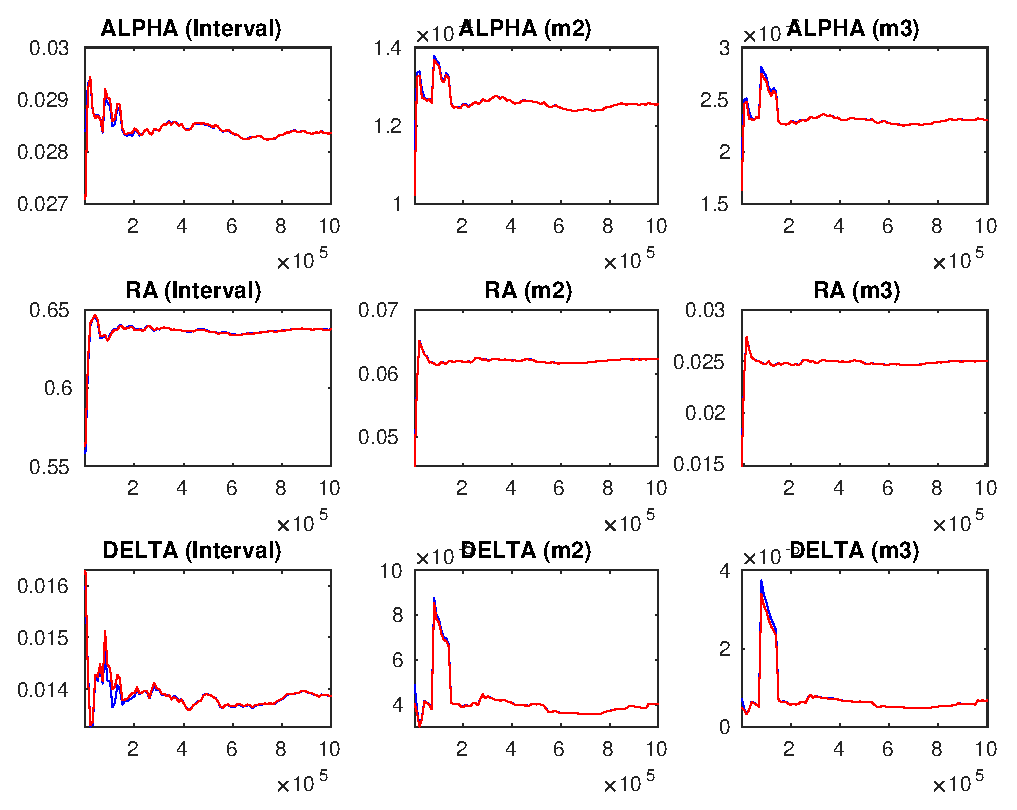
\includegraphics[width=0.80\textwidth]{KimModTheBuilder/Output/KimModTheBuilder_udiag1}
\caption{Univariate convergence diagnostics for the Metropolis-Hastings.
The first, second and third columns are respectively the criteria based on
the eighty percent interval, the second and third moments.}\label{Fig:UnivariateDiagnostics:1}
\end{figure}

\begin{figure}[H]
\psfrag{RHOA (m3)}[1][][0.5][0]{$ {\rho_A} $}
\psfrag{SIGA (Interval)}[1][][0.5][0]{$ {\sigma_A} $}
\psfrag{SIGA (m2)}[1][][0.5][0]{$ {\sigma_A} $}
\psfrag{SIGA (m3)}[1][][0.5][0]{$ {\sigma_A} $}
\psfrag{THETA (Interval)}[1][][0.5][0]{$ {\theta} $}
\psfrag{THETA (m2)}[1][][0.5][0]{$ {\theta} $}
\psfrag{THETA (m3)}[1][][0.5][0]{$ {\theta} $}
\centering 
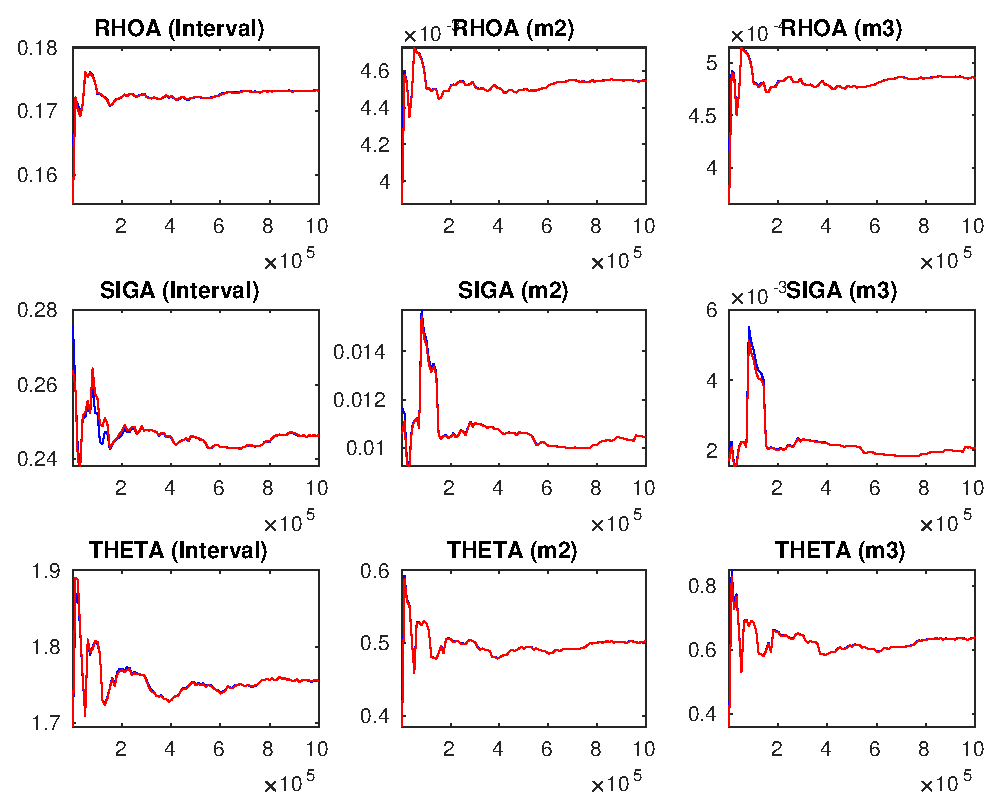
\includegraphics[width=0.80\textwidth]{KimModTheBuilder/Output/KimModTheBuilder_udiag2}
\caption{Univariate convergence diagnostics for the Metropolis-Hastings.
The first, second and third columns are respectively the criteria based on
the eighty percent interval, the second and third moments.}\label{Fig:UnivariateDiagnostics:2}
\end{figure}

\begin{figure}[H]
\psfrag{KAPPA (m3)}[1][][0.5][0]{$ {\kappa} $}
\psfrag{RHOUPSILON (Interval)}[1][][0.5][0]{$ {\rho_\upsilon} $}
\psfrag{RHOUPSILON (m2)}[1][][0.5][0]{$ {\rho_\upsilon} $}
\psfrag{RHOUPSILON (m3)}[1][][0.5][0]{$ {\rho_\upsilon} $}
\psfrag{SIGUPSILON (Interval)}[1][][0.5][0]{$ {\sigma_\upsilon} $}
\psfrag{SIGUPSILON (m2)}[1][][0.5][0]{$ {\sigma_\upsilon} $}
\psfrag{SIGUPSILON (m3)}[1][][0.5][0]{$ {\sigma_\upsilon} $}
\centering 
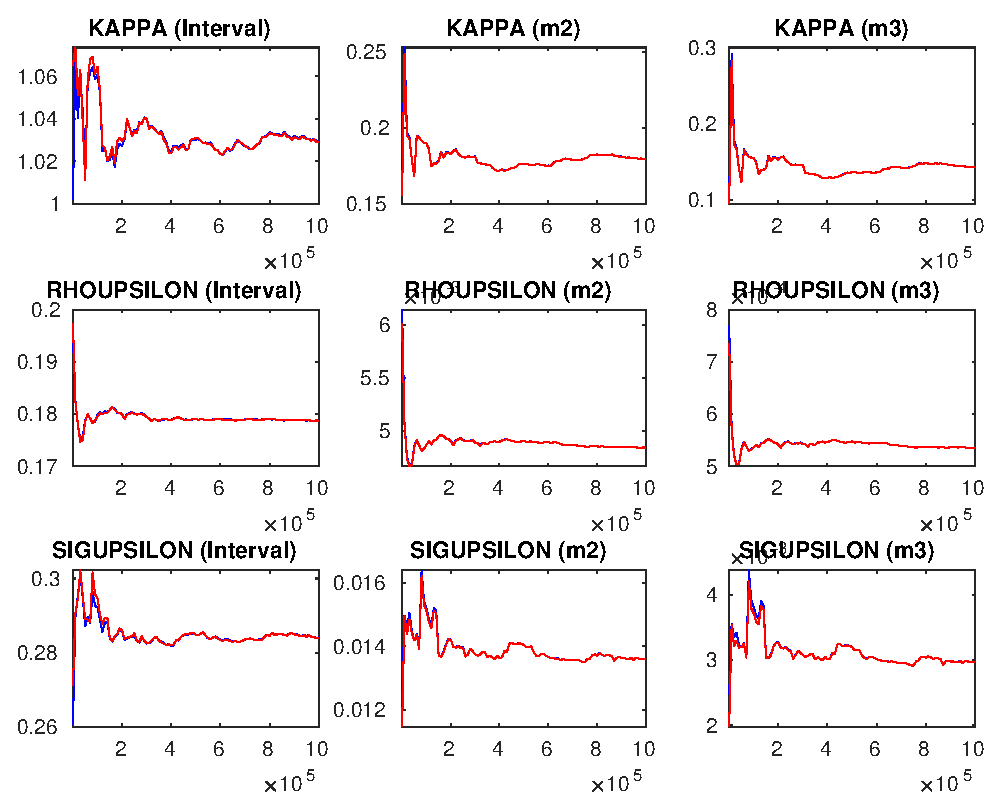
\includegraphics[width=0.80\textwidth]{KimModTheBuilder/Output/KimModTheBuilder_udiag3}
\caption{Univariate convergence diagnostics for the Metropolis-Hastings.
The first, second and third columns are respectively the criteria based on
the eighty percent interval, the second and third moments.}\label{Fig:UnivariateDiagnostics:3}
\end{figure}

